\documentclass[tc, manuscript]{copernicus}

%% \usepackage commands included in the copernicus.cls:
%\usepackage[german, english]{babel}
%\usepackage{tabularx}
%\usepackage{cancel}
%\usepackage{multirow}
%\usepackage{supertabular}
%\usepackage{algorithmic}
%\usepackage{algorithm}
%\usepackage{amsthm}
%\usepackage{float}
%\usepackage{subfig}
%\usepackage{rotating}

\usepackage{booktabs}
\usepackage{multirow}
% \usepackage{datetime}

\begin{document}

\title{Fountain scheduling strategies to improve water use efficiency of artificial
ice reservoirs (Icestupas)}

\def\Authors{Suryanarayanan Balasubramanian\,$^{1}$, Roger Waser\,$^{2}$, Martin Hoelzle\,$^{1}$}
\def\Address{$^{1}$University of Fribourg, Department of Geosciences, Fribourg, Switzerland $^{2}$University of
Applied Sciences and Arts, Luzern, Switzerland} \def\corrAuthor{Suryanarayanan Balasubramanian}
\Author[1]{Suryanarayanan Balasubramanian}{Balasubramanian}
\Author[1]{Martin Hoelzle}{Hoelzle}
\Author[2]{Roger Waser}{Waser}
\affil[1]{University of Fribourg, Department of Geosciences, Fribourg, Switzerland}
\affil[2]{University of Applied Sciences and Arts, Luzern, Switzerland}

\correspondence{suryanarayanan.balasubramanian@unifr.ch}

\runningtitle{Scheduling AIR fountains}

\runningauthor{S. Balasubramanian}

\firstpage{1}

\maketitle

\begin{abstract}

  Automated fountain scheduling can be used to improve Artificial Ice Reservoir (AIR) construction efficiency by
  reducing fountain wastewater production. Mass balance experiments have shown that over 80 \% of the water
  sprayed during traditional AIR construction can be lost. This result gives an indication of the potential
  improvement in water use efficiency that can be achieved by optimising the fountain discharge rate. Improved
  fountain scheduling was realized using an automation system that computes recommended discharge rates using
  real-time weather inputs and location metadata. During the winter of 2021-22, a traditional and an automated
  AIR were built in Guttannen with the main aim of comparing and quantifying the benefits of using automation
  systems. The water requirement for the automated AIR was 87 \% lesser than the traditional AIR. Ice volume
  estimates validated with drone measurements indicate that the automated AIR also achieved higher volumes
  inspite of the reduced discharge rates. Automated AIR simulations when compared with traditional AIR in other
  construction locations yield water use efficiency over 90 \%. Overall, our results show that the automated
  fountain scheduling method increased the water use efficiency of AIR construction 5 fold.

\end{abstract}

\introduction

Artificial Ice Reservoirs (AIRs) have recently received much attention in the light of increasing users,
especially in semi-arid and arid mountain regions facing limited water availability and at the same time
increased water needs. However, their water use efficiency is very poor. 

Fountain scheduling methods are one option for reducing watering volumes for AIR construction systems and, at
the same time, increase water use efficiency. The goal of fountain scheduling is to make the most efficient use of water by
spraying the right amount of water at the right time, making sure water is available when the AIR surface can
freeze it. Scheduling maximizes AIR water use efficiency by minimizing fountain waste water.  

Proper fountain scheduling requires answers to two questions: (a) When should the water be turned on and off?
(b) How much water should be sprayed? Knowledge of surface freezing rates is important for answering these
questions. Surface freezing rates can be calculated by means of two different approaches: physical
and empirically based models. The former may be defined as a model in which each of the relevant
energy fluxes at the AIR surface is computed from physically based calculations using direct measurements of the
necessary meteorological variables, and the freezing rate is calculated as the sum of the individual fluxes
scaled with the AIR surface area during the accumulation period. The latter may be defined as a model in which
the freezing rate is calculated based on an assumed relationship with weather and location parameters. In order
to produce recommended discharge rates, empirical models are preferred due to their parsimony in data
requirement and computational time in comparison with the more sophisticated energy-balance models. But only
physical energy balance models exist for AIRs. Therefore, we present an empirical model that seeks a balance
between model complexity and data availablity.

The main interest in using model results is to simulate alternative fountain schedules relative to various
constrains in monetary investments, construction duration as well as in water availability. The fountain
scheduling alternatives are evaluated from the relative water use efficiency and maximum ice volume produced
during the accumulation period. The specific objectives of this paper include the presentation of the automation
system and examples of its application to the computation of fountain scheduling strategies.

\section{Study site and data}

The Guttannen site (46.66 $\degree$N, 8.29 $\degree$E) in the Bern region lies at 1047 $m$ a.s.l.. In the winter
(Oct-Apr), mean daily minimum and maximum air temperatures vary between -13 and 15 $\degree C$. Clear skies are
rare, averaging around 7 days during winter. Daily winter precipitation can sometimes be as high as 100 $mm$.
These values are based on 30 years of hourly weather model simulations \citep{guttannen}. Two AIRs were
constructed here by the Guttannen Bewegt Association respectively during the winters of 2020-21 using a
traditional and an automated construction strategy.

\begin{figure}[t]
\includegraphics[width=8.3cm]{Figures/2AIRs.jpg}
\caption{Automated and traditional AIRs at Guttannen on February 6, 2022. Picture credits: Daniel Bürki}
\label{fig:2AIR} 
\end{figure}

In order to compare both the construction strategies, the automated and the traditional AIRs were constructed
adjacent to each other as shown in in Fig. \ref{fig:2AIR}. This ensured both AIRs shared the same water source
and similar weather patterns. In addition, a webcam guaranteed a continuous survey of the automated AIR.   

In the traditional strategy, tree branches were laid covering the fountain pipe to initiate the ice formation
process. The fountain discharge was maintained at maximum and its height was increased from 3 to 6\,$m$ during
the construction period.

In the automated strategy, only the fountain pipe was erected before initiation of water spray. An automation
system controlled the fountain discharge rate using real time weather input and several parameters exposed via
the user interface. 

\subsection{Meteorological data}
Air temperature, relative humidity, wind speed, pressure, longwave, shortwave direct and diffuse radiation are
required to calculate the surface energy balance of an AIR (see Fig. ). The construction period starts when the
fountain was first switched on and ends when the fountain was last switched off. These two dates are denoted as
start and fountain off dates henceforth.


\begin{figure*}[t]
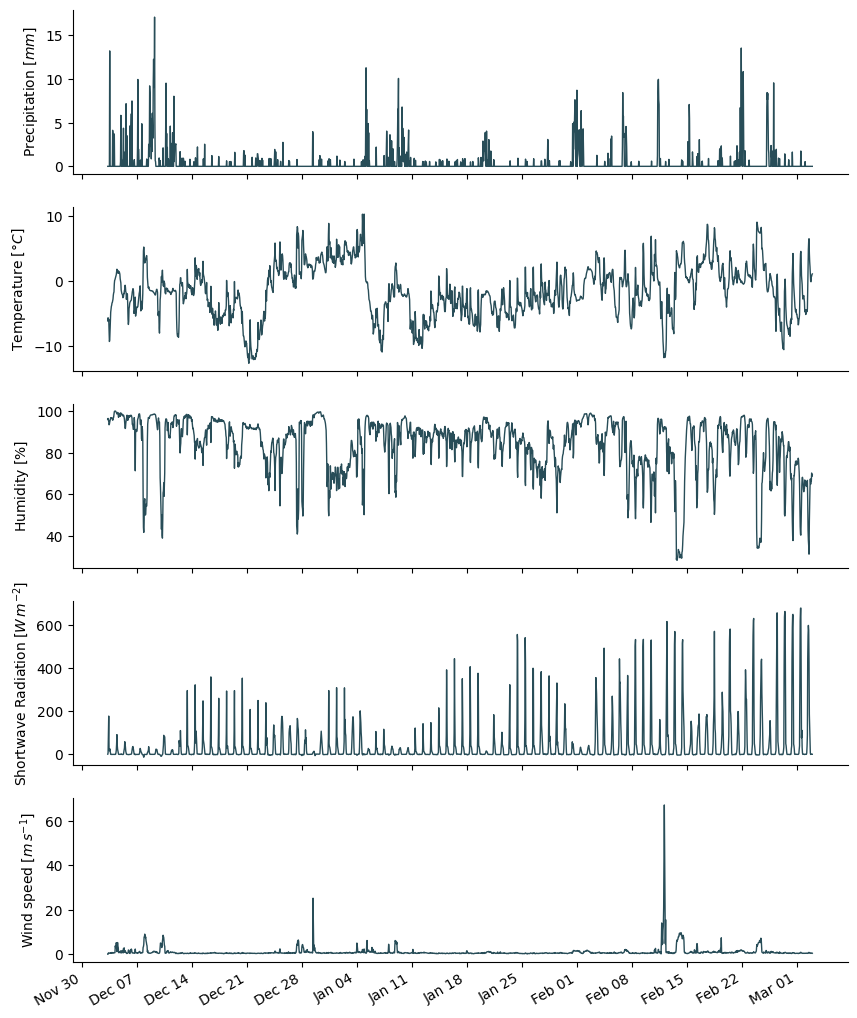
\includegraphics[width=12cm]{Figures/input.png}
\caption{TEXT}
\end{figure*}

The primary weather data source was a automatic weather station (AWS) located around 20 meters away as shown in
Fig. . In addition, we used ERA5 reanalaysis dataset for filling data gaps and adding the shortwave and longwave
radiation data that were not measured directly. The ERA5 reanalysis dataset is known to have a high correlation
with sites in Switzerland (). The Guttannen temperature dataset had a correlation greater the ? with the ERA5
temperature. The ERA5 grid point chosen () for the Guttannen site was around 3.6 km away from the actual site.
ERA5 variables were fitted to the AWS data via linear regressions. 

\subsection{Fountain observations}
We define the fountain used through four attributes; namely, its spray radius, discharge rate, height and water
temperature. The spray radius $r_F$ was estimated from the mean AIR circumference
measured in the drone surveys during the fountain runtime. 

Measurements of the discharge rate for the automated fountain were used to determine the mean discharge of the
traditional fountain. A new fountain design was used for the automated strategy since the traditional fountain
design was unable to function in the whole range of discharge rates suggested by the automation system.

\subsection{Drone surveys}
Several photogrammetric surveys were conducted on the traditional and the automated AIRs. The details of these
surveys and the methodology used to produce the corresponding outputs are explained in the Appendix. The digital
elevation maps (DEMs) generated from the obtained imagery were analysed to document the radius, surface area and
volume of the ice structures. The number of surveys conducted for the traditional and the automated AIRs were
? and ? respectively (see Table). The last drone flight was used to set the dome volume for the traditional AIR.
The dome volume for the automated AIR was zero.  The remaining surveys were used for model validation.

\section{Methods}

\subsection{Automation system}
The automation system implements fountain scheduling strategies for the twin objectives of ice volume (ICV) and water
use efficiency (WUE). The ice volume objective is attractive in locations with sufficient water volumes to
freeze during the construction period. The water use efficiency objective is attractive in locations with
favourable weather conditions constrained by available water supply. For the ICV objective, the model assumptions
overestimate the freezing rate whereas for the WUE objective the model assumptions underestimate the freezing
rate. 

The automation hardware consists of a weather station, flowmeter, control valve, drain valves, air valves,
fountain, pipeline and a logger. The logger feeds the weather station data to the automation software and
informs the recommended discharge rate to the flowmeter. The flowmeter adjusts the control valve to match the
recommendation. In case the recommendation is below the critical discharge rate of the fountain, the drain and
air valves empty the water in the pipeline to prevent any freezing events. Here the critical discharge rate is
defined as the discharge rate below which the fountain pipeline can freeze.

% \begin{figure}[ht]
% 	\begin{center}
% 		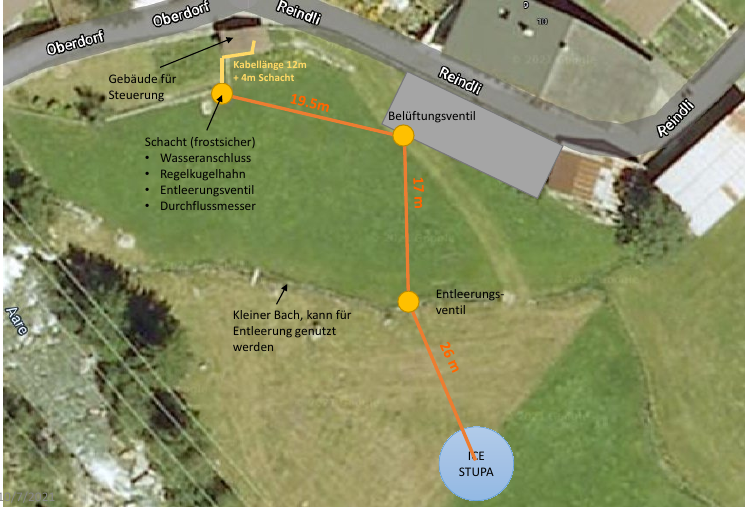
\includegraphics[width=\linewidth]{Figures/automation_system.png}
% 	\end{center}
%   \caption{Guttannen automation system}
% 	\label{fig:layout}
% \end{figure}

The software performs the computations in the least (a) data demanding and (b) computationally intensive way
possible. Objective (a) is achieved by introducing assumptions to the energy balance model as described in the
Appendix . Objective (b) is achieved by formulating a surrogate empirical model that best approximates the
simplified physical model. 


\begin{table}[]
\centering
\caption{Assumptions introduced to simplify the model.}
\label{tab:assumptions}
\begin{tabular}{@{}lllll@{}}
\toprule
\textbf{Objective} & \textbf{Symbol} & \textbf{Ice Volume} & \textbf{WUE} & \\ \midrule
\multicolumn{1}{|l}{Surface Area}        & $A_{cone}$ & $ \sqrt{2} \pi r_{F}^2$ & $\pi r_{F}^2$ & \multicolumn{1}{l|}{} \\ \midrule
\multicolumn{1}{|l}{Shortwave Radiation} & $q_{SW}$ & $cld = 0$ ; $\alpha=\alpha_{ice}$; & $cld = 1$ ;
$\alpha=\alpha_{snow}$; & \multicolumn{1}{l|}{} \\ 
\multicolumn{1}{|l}{ } &  & $f_{cone} = \frac{cos \theta_{sun} + \pi sin \theta_{sun}}{2\sqrt{2}\pi}$  & $f_{cone} = sin \theta_{sun} / 2$ & \multicolumn{1}{l|}{} \\ \midrule
\multicolumn{1}{|l}{Longwave Radiation}  & $q_{LW}$ & $cld = 0$ ; $T_{ice} = 0$ & $cld = 1$ ; $T_{ice} = 0$ & \multicolumn{1}{l|}{} \\ \midrule
\multicolumn{1}{|l}{Sensible and Latent Heat}       & $q_{S}$ &$\mu_{cone} = 1.5$  & $\mu_{cone} = 1$ & \multicolumn{1}{l|}{} \\ \midrule
\multicolumn{1}{|l}{Temperature heat flux} & $q_{T}$ & 0 & 0 & \multicolumn{1}{l|}{} \\ \midrule
\multicolumn{1}{|l}{Fountain discharge heat flux} & $q_{F}$ & 0 & 0 & \multicolumn{1}{l|}{} \\ \midrule
\multicolumn{1}{|l}{Ground heat flux}    & $q_{G}$ & 0 & 0 & \multicolumn{1}{l|}{} \\ \bottomrule
\end{tabular}
\end{table}

For objective (b), we approximate the shortwave radiation flux into a gaussian equation with three coefficients
and the rest of the heat flux components into a linear equation with 4 coefficients. The coefficients of the
shortwave gaussian function $g($ hour of day $)$ are calibrated based on estimation of solar radiation during
the last day of the construction period. We approximate the rest of the energy fluxes by assuming a linear
relationship with the weather parameters namely, temperature, humidity, wind speed and altitude. Using the above
simplifications, we can compute the expected thickness change rates using the following set of equations:

\begin{subequations}
	\begin{align}
		\label{eqn:sun}
  \frac{q_{SW}}{\rho_w \cdot L_F} & \approx \frac{amp}{(\sigma \sqrt{2\pi})} \cdot
  exp\left(\frac{-(hod-\mu)^2}{2\sigma^2}\right) = g(hod)  \\
		\label{eqn:T}
   \frac{q_{LW} + q_{S}}{\rho_w \cdot L_F} + \frac{q_L}{\rho_w \cdot L_V} & \approx a \cdot T_a + b \cdot RH + c \cdot v_a +
  d \cdot alt + e = f(T_a, RH, v_a, alt) \\
		\label{eqn:auto}
  \frac{\Delta j_{cone}}{\Delta t} & \approx g(hod) + f(T_a, RH, v_a, alt)\\
		\label{eqn:auto}
  \frac{\Delta Q_{F}}{\Delta t} & \approx \frac{\Delta j_{cone}}{\Delta t} \cdot \pi r_{F}^2 \cdot
  \frac{1000}{60}
	\end{align}
\end{subequations}

where $r_F$ is the fountain spray radius, $\frac{\Delta j_{cone}}{\Delta t}$ is the thickness change rate,
$\frac{\Delta Q_{F}}{\Delta t}$ is the discharge rate and $hod$ is the hour of day.

% \begin{table}[ht]
% \centering
% \caption{}
% \label{tab:my-table}
% \begin{tabular}{@{}lllllllll@{}}
% \toprule
% Coefficients  & $T_a\, [\degree C]$ & $RH\,[\%]$ & $v_a\, [m\, s^{-1}]$ & $alt\, [km]$  & $constant$ \\ \midrule
% Coefficients  & $a$ & $b$ & $c$ & $d$  & $e$ & $amp$ & $\mu$ & $\sigma$ \\ \midrule
% Value           & $\num{-5.6 e-3}$     & $\num{-3.2 e-4}$ & $\num{4.7 e-3}$ & $\num{-3.5 e-3}$  & $\num{5.2
% e-3}$ & $\num{5.2 e-3}$ & $\num{5.2 e-3}$ & $\num{5.2 e-3}$  \\ \bottomrule
% \end{tabular}
% \end{table}

The software is configured in such a way that it works independently of a PC. Once switched on, the software
starts automatically. The system runs if none of the following termination criteria apply:

\begin{itemize}
\item Wind speed greater than limit value
\item Ambient temperature higher or lower than limit values
\item Pipeline freezing event detected: $IW_{KH} > 20 \%$ and $Q_w = 0$ for atleast 20 seconds (Icing)
\item Leakage detected: $Q_w > 65 l/min$
\end{itemize}

% \begin{figure}[ht]
% 	\begin{center}
% 		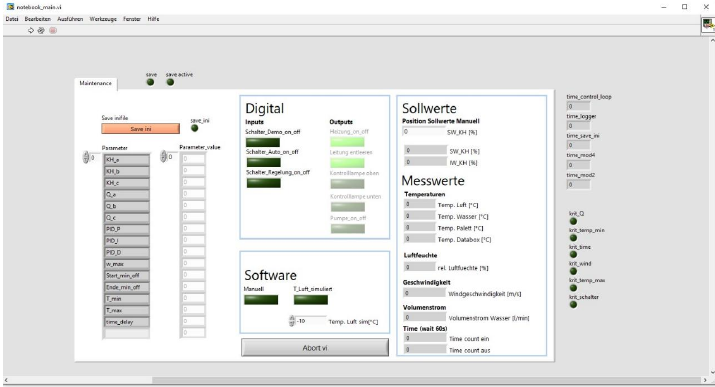
\includegraphics[width=\linewidth]{Figures/user_interface.png}
% 	\end{center}
%   \caption{User Interface}
% 	\label{fig:UI}
% \end{figure}

\subsection{Model calibration}
\subsection{Model comparison and validation}
The success of the empirical model in approximating the physical model is judged using the efficiency criteria,
$R^2$, (Nash and Sutcliffe,1970) of the empirically and physically estimated freezing rates, $Q_{phy/emp}$: 

\begin{equation}
  R^2 = 1 - \frac{\Sigma(Q_{phy} - Q_{emp})^2}{\Sigma(Q_{phy} - Q_{phy})^2}
\end{equation}

An $R^2$ of 1 indicates perfect fit; $R^2<0$ indicates that the average value of all observations is a better
predictor than the model itself. 

For the physical model validation, simulated and observed ice volume changes are compared.

\section{Results}

\subsubsection{Shortwave radiation comparison}

\subsubsection{Freezing rate comparison}

\subsection{Ice Volume Validation}

% \begin{figure}[ht]
% 	\begin{center}
% 		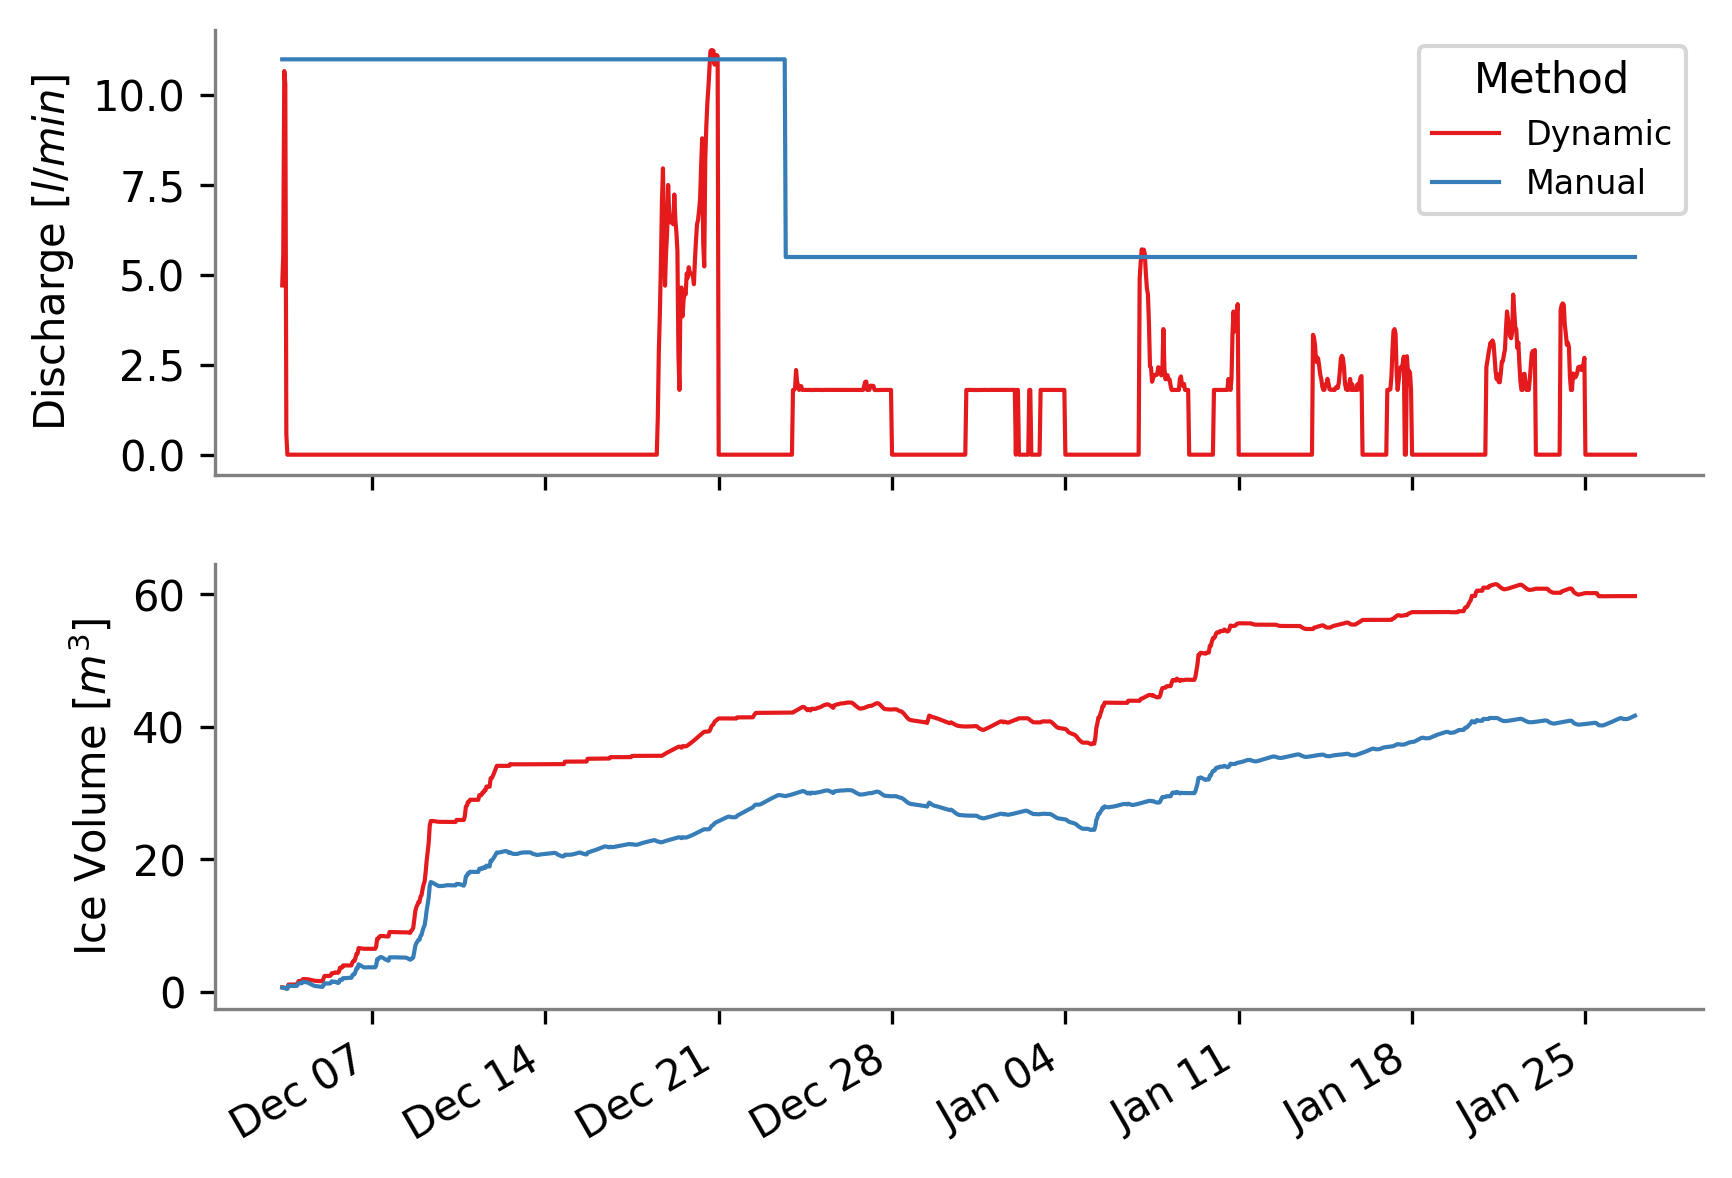
\includegraphics[width=\linewidth]{Figures/autovsman_dis.png}
% 	\end{center}
% 	\caption{Comparison of discharge and ice volume between AIRs produced by dynamic and static fountains. }
% 	\label{fig:old_icestupa}
% \end{figure}


\subsection{Water Use efficiency}

% \begin{figure}[ht]
% 	\begin{center}
% 		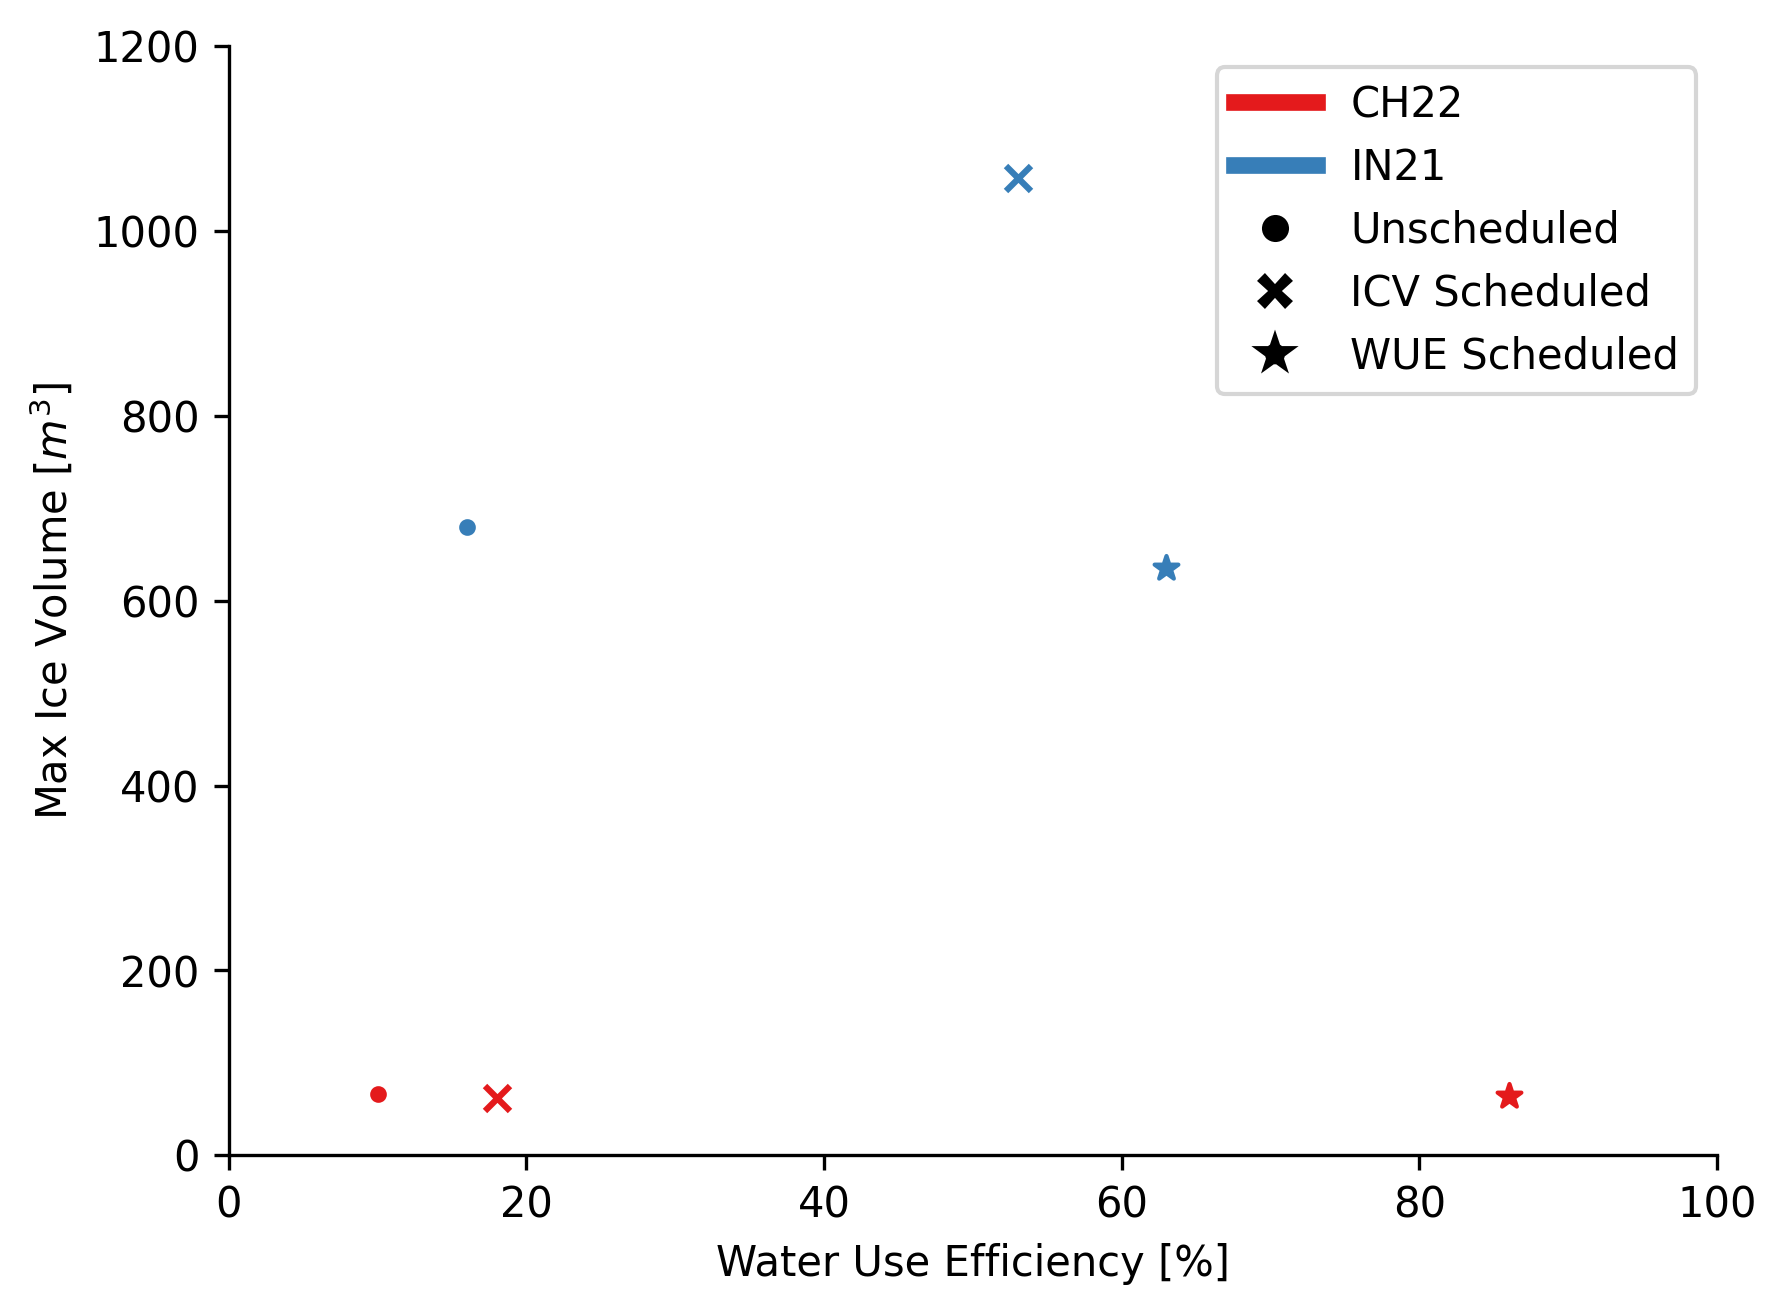
\includegraphics[width=\linewidth]{Figures/wue.png}
% 	\end{center}
% 	\caption{Comparison of discharge and ice volume between AIRs produced by dynamic and static fountains. }
% 	\label{fig:old_icestupa}
% \end{figure}

\section{Discussion}
\subsection{Fountain vs weather influence}

\subsection{Ideal fountains and locations for AIR construction}

\subsection{Fountain height and spray radius}

% \subsection{Eddy covariance comparison}

\subsection{Surface temperature}

\subsection{Implementation costs}

Since this technology is currently being used by subsistence farmers, we also need to be mindful of the
maintenance and implementation costs. We propose two different modes of fountain scheduling based on operation
costs that can be classified as static or dynamic. In the static mode, the total amount of water
for AIR construction is allocated without specifying its temporal distribution along the accumulation period. By
contrast, in the dynamic mode water is allocated at specific time steps along the accumulation period in
order to achieve even higher WUE.

Both the approaches use a fountain and pipeline system with minimal manual intervention. The dynamic mode is
better suited for locations where the diurnal and seasonal variations in the weather conditions are significant.
In such cases, the real-time adjustments of the discharge rate make efficient fountain scheduling
possible. The static mode is better suited for other locations or for users who cannot afford the additional
hardware requirements to implement the dynamic fountain scheduling mode.

\conclusions

In this paper, two different construction strategies that yield better water use efficiency are presented.
An automation system was developed to implement the dynamic fountain sischarge mode and tested using data
collected at Guttannen, Switzerland during the 2021-22 winter season. 

The main purpose of this study was to test the idea that scheduling AIR fountain systems could lead to a
significant improvement in water use efficiency.

This study has demonstrated the importance of fountain scheduling. Furthermore, the decrease in performance of
the empirical model has been quantified through comparison of efficiency criteria. The study has demonstrated
that, it is possible to compute more than 90 \% of the freeze rate variations by means of a simplified empirical
model. This model satisfies the need for a less data demanding and computationally intensive workflow for
scheduling fountains worldwide using the computation of just 6 coefficents. Such a model will be compatible with
the limited data amount that is typical of any new AIR construction location.

This study has also compared the sensitivity of freezing rates between the weather components and the fountain's
spray radius. It is clear that if improvements are to be achieved, future research must be devoted to modelling
the impact of fountain design on the spray radius.

The model discussed in this paper will be applied worldwide to identify favourable AIR locations in a future
paper.


The automation system allows the easy handling of fountain scheduling implementation. Its capabilities for
achieving a higher water saving was tested for Guttannen. The possibility for easily changing the automation
coefficients allows tailoring the fountain discharge rate according to identified requirements. Other on-going
improvements concern the use of the automation software as a decision support tool applicable at both the local
and the global scale.



\appendix

\section{Simplified energy balance model}

We approximate the energy balance at the surface of an AIR by a one-dimensional description of energy fluxes as
used in \cite{balasubramanianInfluenceMeteorologicalConditions2022}. The ice volume evolution of the AIR can be
represented as: 

\begin{equation}
  \frac{\Delta V_{ice}}{\Delta t}  =  \frac{\Delta j_{cone}}{ \Delta t} \cdot A_{cone}
	\label{eqn:freeze}
\end{equation}

where $\frac{\Delta j_{cone}}{\Delta t}$ is the thickness change determined as follows:

\begin{equation}
  \frac{\Delta j_{cone}}{\Delta t}  = \frac{1}{\rho_w} \cdot (\frac{q_{SW} + q_{LW} + q_{S} + q_{F} + q_{G} -
  q_{T}}{L_F} + \frac{q_{L}}{L_V} )
	\label{eqn:freeze}
\end{equation}

Upward and downward fluxes relative to the ice surface are positive and negative, respectively. The first term
represents the surface thickness change rate due to freezing of the fountain water and melting of the ice.
$q_{SW}$ is the net shortwave radiation; $q_{LW}$ is the net longwave radiation; $q_{L}$ and $q_{S}$ are the
turbulent latent and sensible heat fluxes; $q_{F}$ is the fountain heat flux; $q_{G}$ is the ground heat flux
and $q_{T}$ is the temperature heat flux. However, we assume $q_{F}$, $q_{G}$ and $q_{T}$ to be negligible.

We reduce the data requirement for estimation of each of the energy flux components in two ways:

\begin{itemize}
  \item Pressure estimation using the location's altitude through the PVLIB model described in
    \citet{holmgrenPvlibPythonPython2018}.
  \item Direct and diffuse shortwave radiation estimation using the location's coordinates and altitude through the
    PVLIB model described in \citet{holmgrenPvlibPythonPython2018}. The algorithm used to estimate the
    clear-sky global radiation is described in \citet{ineichenBroadbandSimplifiedVersion2008} and the algorithm
    used to estimate the diffuse part of the global radiation is described in
\citet{erbsEstimationDiffuseRadiation1982}. The uncertainty of this approach is discussed in
\cite{ineichenValidationModelsThat2016}. 
\end{itemize}

The model complexity was reduced through assumptions that optimise for the ice volume objective or the water use
efficiency objective. Assumptions are chosen based on whether they overestimate/underestimate the freezing rate.
Ice volume objective requires freezing rate to be overestimated whereas WUE objective requires freezing rate to
be underestimated. We describe these two kinds of assumptions applied on each of the energy balance components
below: 

\subsection{Surface Area $A_{cone}$ assumptions}

Since we are only interested in determination of the surface area during the accumulation period we can assume a
constant ice cone radius equal to the fountain spray radius. The surface area scales the freezing rate of the
AIR. Hence, for the IceV objective we assume the maximum possible slope of 1 for the ice cone or in other words
$h_{cone} = r_{F}$. Similarly, for the WUE objective, the area of the conical AIR is
approximated to the area of its circular base. 

\begin{equation} A_{cone} =\pi \cdot r_{F}^2 \label{eq:Area} \end{equation}

\subsection{Net shortwave radiation \texorpdfstring{$q_{SW}$}{Lg} assumptions}
\label{sec:SW}

The net shortwave radiation $q_{SW}$ is computed as follows:

\begin{equation} q_{SW} = (1- \alpha) \cdot ( SW_{direct} \cdot f_{cone} + SW_{diffuse})
\label{eqn:SW} \end{equation}

where $\alpha$ is the albedo value ; $SW_{direct}$ is the direct shortwave radiation; $SW_{diffuse}$ is the
diffuse shortwave radiation and $f_{cone}$ is the solar area fraction.

The diffuse and direct shortwave radiation is determined using the estimated global solar radiation as follows:

\begin{equation}
\begin{split}
  SW_{diffuse} &= cld \cdot SW_{global}\\
  SW_{direct} &= (1-cld) \cdot SW_{global}
\end{split}
\end{equation}

where $cld$ is the cloudiness factor. $cld$ is assumed to be 1 and 0 for the WUE and iceV objective
respectively.

We ignore the variations in the albedo and assume it to be equal to snow albedo and ice albedo for the iceV and
WUE objective respectively. 

The solar area fraction $f_{cone}$ of the ice structure exposed to the direct shortwave radiation depends on the
shape considered. It is computed as

\begin{equation}
		f_{cone} =\frac{(0.5 \cdot r_{cone} \cdot h_{cone}) \cdot cos \theta_{sun} +(\pi \cdot
			{(r_{cone})}^2/2) \cdot sin \theta_{sun} }{\pi \cdot r_{cone} \cdot ({(r_{cone})}^2+{(h_{cone})}^2)^{1/2}}\\
\end{equation}

For the IceV objective, since we assume the slope of the cone to be 1 $f_{cone}$ is determined
as follows:

\begin{equation}
		f_{cone} =\frac{ cos \theta_{sun} + \pi \cdot sin \theta_{sun} }{2\sqrt{2} \cdot \pi }
\end{equation}

Similarly, for the WUE objective, since we assume the slope of the cone to be negligible, we get:

\begin{equation}
		f_{cone} =\frac{ sin \theta_{sun} }{2 }
\end{equation}


\subsection{Net Longwave radiation \texorpdfstring{$q_{LW}$}{Lg} assumptions} \label{sec:LW}


We assume $T_{ice} = 0 \degree C$ in order to determine outgoing longwave radiation. Since it is challenging to
contrain the minimum ice temperature, we maintain this assumption for both our objectives. However, in order to
estimate atmospheric emissivity we again assume $cld$ to be 1 and 0 for the WUE and iceV objective respectively.

\subsection{Turbulent fluxes assumptions} \label{sec:Qs}

Turbulent fluxes estimation depend on the slope of the cone through the $\mu_{cone}$ parameter. As suggested 
by \citet{oerlemansBriefCommunicationGrowth2021}, we can estimate this parameter as follows:

\begin{equation}
  \mu_{cone} =1 + s_{cone}/2
\end{equation}

Hence, the $\mu_{cone}$ parameter takes values of 1.5 and 1 for the iceV and WUE objective respectively.  Since
turbulent fluxes impact both the freezing and the melting rates, this assumption may not favor the corresponding
objectives for certain sites.

\noappendix       %% use this to mark the end of the appendix section. Otherwise the figures might be numbered incorrectly (e.g. 10 instead of 1).

\bibliographystyle{copernicus}
\bibliography{zot_refs.bib}

\end{document}

%% Regarding figures and tables in appendices, the following two options are possible depending on your general handling of figures and tables in the manuscript environment:

%% Option 1: If you sorted all figures and tables into the sections of the text, please also sort the appendix figures and appendix tables into the respective appendix sections.
%% They will be correctly named automatically.

%% Option 2: If you put all figures after the reference list, please insert appendix tables and figures after the normal tables and figures.
%% To rename them correctly to A1, A2, etc., please add the following commands in front of them:

\appendixfigures  %% needs to be added in front of appendix figures

\appendixtables   %% needs to be added in front of appendix tables

%% Please add \clearpage between each table and/or figure. Further guidelines on figures and tables can be found below.
age between each table and/or figure. Further guidelines on figures and tables can be found below.

%% LITERATURE CITATIONS
%%
%% command                        & example result
%% \citet{jones90}|               & Jones et al. (1990)
%% \citep{jones90}|               & (Jones et al., 1990)
%% \citep{jones90,jones93}|       & (Jones et al., 1990, 1993)
%% \citep[p.~32]{jones90}|        & (Jones et al., 1990, p.~32)
%% \citep[e.g.,][]{jones90}|      & (e.g., Jones et al., 1990)
%% \citep[e.g.,][p.~32]{jones90}| & (e.g., Jones et al., 1990, p.~32)
%% \citeauthor{jones90}|          & Jones et al.
%% \citeyear{jones90}|            & 1990


%% FIGURES

%% When figures and tables are placed at the end of the MS (article in one-column style), please add \clearpage
%% between bibliography and first table and/or figure as well as between each table and/or figure.

% The figure files should be labelled correctly with Arabic numerals (e.g. fig01.jpg, fig02.png).


%% ONE-COLUMN FIGURES

%%f
%\begin{figure}[t]
%\includegraphics[width=8.3cm]{FILE NAME}
%\caption{TEXT}
%\end{figure}
%
%%% TWO-COLUMN FIGURES
%
%%f
%\begin{figure*}[t]
%\includegraphics[width=12cm]{FILE NAME}
%\caption{TEXT}
%\end{figure*}
%
%
%%% TABLES
%%%
%%% The different columns must be seperated with a & command and should
%%% end with \\ to identify the column brake.
%
%%% ONE-COLUMN TABLE
%
%%t
%\begin{table}[t]
%\caption{TEXT}
%\begin{tabular}{column = lcr}
%\tophline
%
%\middlehline
%
%\bottomhline
%\end{tabular}
%\belowtable{} % Table Footnotes
%\end{table}
%
%%% TWO-COLUMN TABLE
%
%%t
%\begin{table*}[t]
%\caption{TEXT}
%\begin{tabular}{column = lcr}
%\tophline
%
%\middlehline
%
%\bottomhline
%\end{tabular}
%\belowtable{} % Table Footnotes
%\end{table*}
%
%%% LANDSCAPE TABLE
%
%%t
%\begin{sidewaystable*}[t]
%\caption{TEXT}
%\begin{tabular}{column = lcr}
%\tophline
%
%\middlehline
%
%\bottomhline
%\end{tabular}
%\belowtable{} % Table Footnotes
%\end{sidewaystable*}
%
%
%%% MATHEMATICAL EXPRESSIONS
%
%%% All papers typeset by Copernicus Publications follow the math typesetting regulations
%%% given by the IUPAC Green Book (IUPAC: Quantities, Units and Symbols in Physical Chemistry,
%%% 2nd Edn., Blackwell Science, available at: http://old.iupac.org/publications/books/gbook/green_book_2ed.pdf, 1993).
%%%
%%% Physical quantities/variables are typeset in italic font (t for time, T for Temperature)
%%% Indices which are not defined are typeset in italic font (x, y, z, a, b, c)
%%% Items/objects which are defined are typeset in roman font (Car A, Car B)
%%% Descriptions/specifications which are defined by itself are typeset in roman font (abs, rel, ref, tot, net, ice)
%%% Abbreviations from 2 letters are typeset in roman font (RH, LAI)
%%% Vectors are identified in bold italic font using \vec{x}
%%% Matrices are identified in bold roman font
%%% Multiplication signs are typeset using the LaTeX commands \times (for vector products, grids, and exponential notations) or \cdot
%%% The character * should not be applied as mutliplication sign
%
%
%%% EQUATIONS
%
%%% Single-row equation
%
%\begin{equation}
%
%\end{equation}
%
%%% Multiline equation
%
%\begin{align}
%& 3 + 5 = 8\\
%& 3 + 5 = 8\\
%& 3 + 5 = 8
%\end{align}
%
%
%%% MATRICES
%
%\begin{matrix}
%x & y & z\\
%x & y & z\\
%x & y & z\\
%\end{matrix}
%
%
%%% ALGORITHM
%
%\begin{algorithm}
%\caption{...}
%\label{a1}
%\begin{algorithmic}
%...
%\end{algorithmic}
%\end{algorithm}
%
%
%%% PHYSICAL UNITS
%%%
%%% Please use \unit{} and apply the exponential notation


\end{document}
